\subsection{Handling Emoji}

Analyzing emoji in Italian tweets is essential for understanding expressiveness, sentiments, and the main topics shared online. Emoji represent a unique form of communication that complements textual language with visual symbols to convey emotions, emphasis, and cultural context. Our objectives are therefore to:
\begin{itemize}
    \item Identify emoji usage patterns in Italian tweets.
    \item Analyze the frequency and distribution of emoji.
    \item Explore the semantic meaning of emoji in relation to textual content.
    \item Apply clustering techniques to categorize tweets based on emoji usage.
\end{itemize}

\subsubsection{Dataset and Preprocessing}
To ensure the quality of the analysis, the dataset was pre-processed using the following steps:
\begin{enumerate}
    \item \textbf{Removal of superfluous elements}: Mentions (\texttt{@user}), URLs, hashtags, and non-decodable characters were removed.
    \item \textbf{Text normalization}: All text was converted to lowercase, and redundant spaces were removed.
    \item \textbf{Tokenization}: The text was separated into individual words or symbols for detailed analysis.
    \item \textbf{Emoji extraction}: The \texttt{emoji} library was used to identify and isolate emoji symbols from the text.
\end{enumerate}

\subsubsection{Extraction and Analysis}
We performed two different extractions — one for emoticons and another for emoji. The former required designing a pattern to identify them, while the latter was handled through tokenization and recognition patterns provided by the \texttt{emoji} library. The following analyses were conducted:
\begin{itemize}
    \item \textbf{Emoji counting}: Calculation of the frequency of each emoji in the dataset.
    \item \textbf{Meaning mapping}: Linking emoji to their descriptive names and semantic meanings.
    \item \textbf{Emoji distribution}: Statistical analysis to identify the most common emoji.
    \item \textbf{Relationship with textual content}: Exploration of the correlation between emoji usage and the topics discussed in tweets.
\end{itemize}

\subsubsection{Visualization and Results}
The main visualizations developed include:
\begin{enumerate}
    \item \textbf{Emoji frequency}: A bar chart showing the most used emoji in the dataset.
    \item \textbf{Clustering}: Use of algorithms such as \texttt{K-Means} and \texttt{PCA} to identify groups of tweets based on common emoji usage patterns.
\end{enumerate}
\begin{figure}
    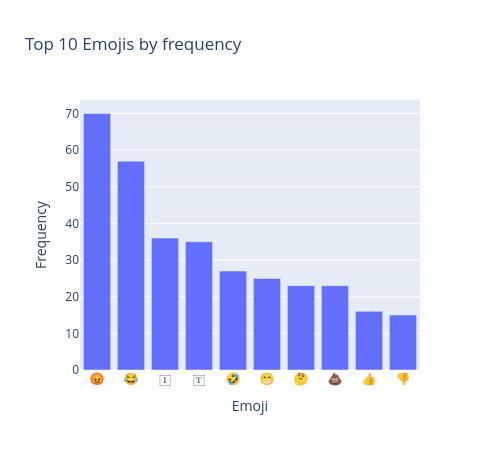
\includegraphics[width=\columnwidth]{../../results/images/emoji_top10.png}
    \caption{Distribution of the most frequent emoji in tweets.}
    \label{fig:emoji_frequenze}
\end{figure}
As we can see from the bar chart, the most frequently used emoji is the enraged face. This visualization provides valuable insight into the trends among the tweets under analysis. As expected, the most prominent sentiment is anger. Subsequent results are also significant, showing the laughing face and then the “IT” pair of emoji. When combined, these emoji might suggest the prevalence of sarcasm, anger, and blame directed toward the government.

\subsubsection{TF-IDF for Emoji and Emoticon Analysis}
One key technique was the use of TF-IDF (Term Frequency–Inverse Document Frequency) to analyze the meaning and importance of both emoji and emoticons in relation to the textual content of the tweets. The process was structured as follows:
\begin{enumerate}
    \item \textbf{Text tokenization}: Each tweet was divided into tokens, including both emoji and emoticons.
    \item \textbf{Generation of n-grams}: For each emoji-emoticon, n-grams (from 1-gram to 5-gram) were generated to analyze combined usage patterns.
    \item \textbf{Frequency calculation}: The relative frequency (TF) of each n-gram was calculated within each tweet.
    \item \textbf{Inverse weighting calculation}: The relative importance of each n-gram in the corpus was calculated, penalizing those present in all tweets (IDF).
    \item \textbf{Vectorization}: Each tweet was represented as a TF-IDF vector, with each dimension corresponding to an n-gram.
    \item \textbf{Parameter optimization}: The optimal value of \textit{n} (the length of the n-grams) was chosen based on total frequency.
\end{enumerate}
Implementing TF-IDF made it possible to distinguish generic symbols with common meanings from those that are more specific and reflective of particular themes or emotions.

\subsubsection{Results of the TF-IDF Analysis}
Applying TF-IDF highlighted the following main n-grams with their corresponding TF-IDF values (cf. Table \ref{tab:tfidf_results}).

\begin{table}[!h]
    \centering
    \begin{tabular}{lc}
    \toprule
    \textbf{N-gram} & \textbf{TF-IDF} \\
    \midrule
    enraged\_face & 0.003181 \\
    italy & 0.002182 \\
    face\_with\_tears\_of\_joy & 0.002172 \\
    thinking\_face & 0.001885 \\
    xo & 0.001316 \\
    pile\_of\_poo & 0.001268 \\
    rolling\_on\_the\_floor\_laughing & 0.001136 \\
    beaming\_face\_with\_smiling\_eyes & 0.001036 \\
    d & 0.001024 \\
    enraged\_face\_enraged\_face & 0.000979 \\
    \bottomrule
    \end{tabular}
    \caption{Top n-grams of emoji names with corresponding TF-IDF values.}
    \label{tab:tfidf_results}
\end{table}

\subsubsection{Comparison of Emoji in Tweets With and Without Hate Speech}
A comparison of the emoji used in tweets with and without hate speech was carried out to analyze differences and specific patterns. The relative frequencies of emoji were calculated in both datasets:
\begin{itemize}
    \item \textbf{Tweets with Hate Speech (HS)}: Includes tweets where \texttt{hs} $= 1$.
    \item \textbf{Tweets without Hate Speech (NHS)}: Includes tweets where \texttt{hs} $= 0$.
\end{itemize}
Emoji frequencies were represented graphically for each group (cf. Figure \ref{fig:hs_emoji}).

\begin{figure}
    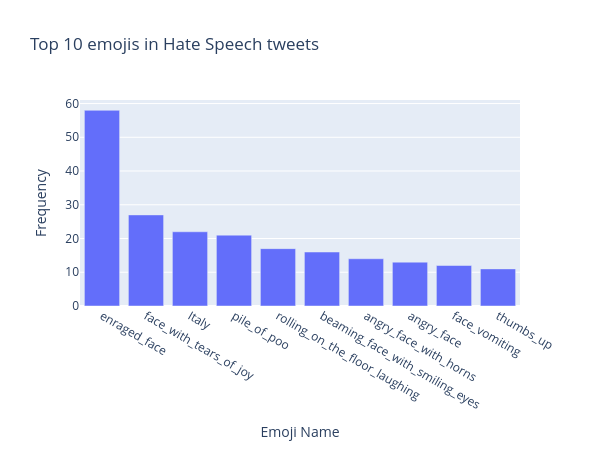
\includegraphics[width=\columnwidth]{../../results/images/emoji_top10_hs.png}
    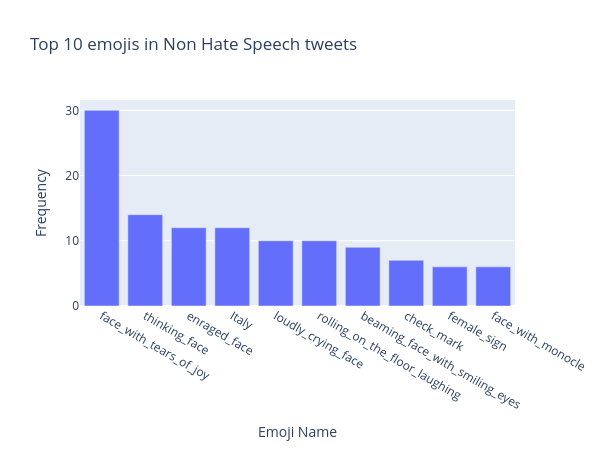
\includegraphics[width=\columnwidth]{../../results/images/emoji_top10_nhs.png}
    \caption{Top 10 Emoji in Tweets With and Without Hate Speech.}
    \label{fig:hs_emoji}
\end{figure}
As we can see in Figure \ref{fig:hs_emoji}, emoji such as “Italy,” “face\_with\_tears\_of\_joy,” “enraged\_face,” etc., appear in both rankings and also at the top positions. This suggests that the enraged face emoji can sometimes be used to express emotions of disappointment, political fatigue, and distrust regarding the topic of immigration. Conversely, the presence of the laughing emoji in the first ranking is indicative of malevolent sarcasm, mockery, and frustration. A similar observation applies to the Italian flag emoji, which is often used in both types of tweets.
\newpage
\subsubsection{Tweet Clustering}
Clustering was performed to categorize tweets based on emoji and emoticons. The main steps were:
\begin{enumerate}
    \item \textbf{Data transformation}: We used the TF-IDF vectors based on the emoji names created before.
    \item \textbf{Determining the optimal number of clusters}: The \textit{Elbow} method was used to find the optimal value of \( k \). Figure~\ref{fig:elbow_method} shows the Elbow method plot.
    \item \textbf{Dimensionality reduction}: \texttt{Principal Component Analysis} (PCA) was applied to reduce the data to three dimensions for visualization.
    \item \textbf{Clustering}: The \texttt{K-Means} algorithm was used to identify four distinct clusters based on emoji usage.
\end{enumerate}

\begin{figure}
    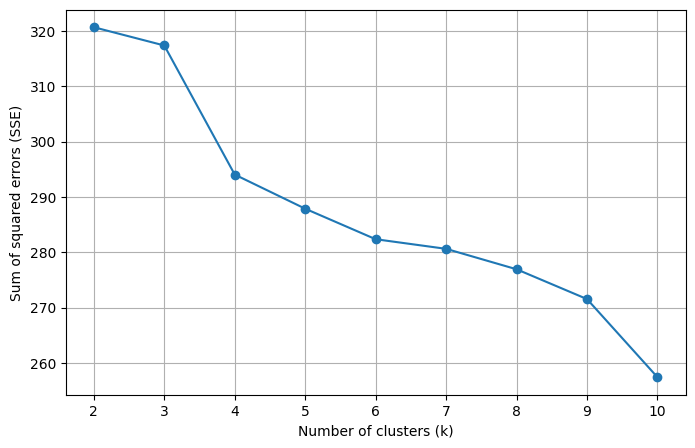
\includegraphics[width=\columnwidth]{../../results/images/emoji_elbow.png}
    \caption{Elbow Method for Determining the Optimal Number of Clusters.}
    \label{fig:elbow_method}
\end{figure}

\begin{figure}
    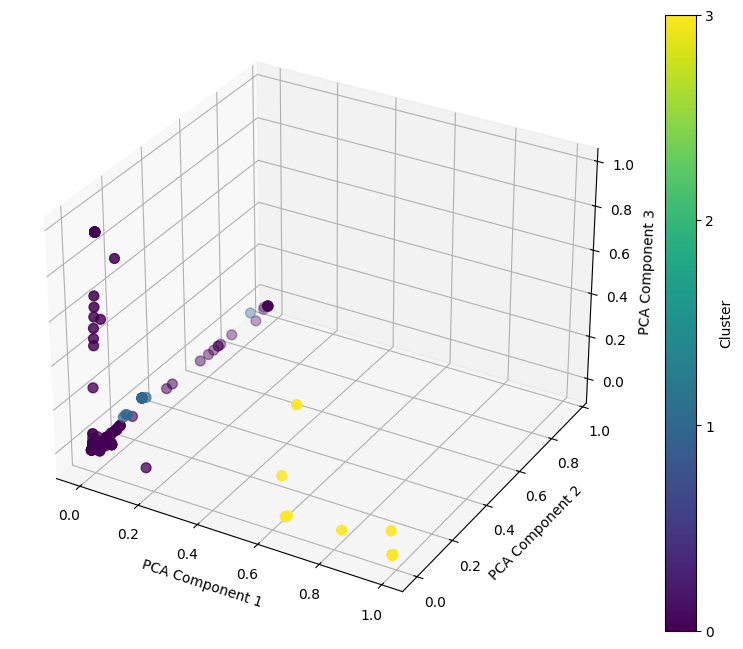
\includegraphics[width=\columnwidth]{../../results/images/emoji_cluster.png}
    \caption{K-Means Emoji Clustering (k=4) – 3D Visualization.}
    \label{fig:3d_clustering}
\end{figure}

Figure~\ref{fig:3d_clustering} shows the cluster distribution in a three-dimensional space based on the computed principal components.

The results show that emoji are not easily clusterable. Even though the optimal \( k \) found is 4, we end up with only 3 actual clusters. This is due to the nature of the available data. The division seems to be on the vertical layer and, based on the trend of the obtained data, we can hypothesize that the blue cluster contains emoji with negative sentiment, the yellow cluster contains those with positive sentiment, and the magenta cluster comprises neutral emoji used in tweets featuring hate speech. These are merely hypotheses, since we are not able to derive more relevant information.
